\section{Implementing sparse DSC on FPGA} \label{sec:implementation}
In the previous section, we detailed how to prune $1 \times 1$ kernels, how the bottleneck convolution is computed, and we analyzed the design hardware variables. In this section, we explore how we can implement the chosen design into an \acrshort{fpga}. The hardware design was implemented using SystemVerilog and the corresponding code can be found at this address: 
%
\begin{center}
    \url{https://github.com/ggheysen/UCL-EPL-Master-Thesis-2019-2020}.
\end{center}
%
According to the scope of this thesis, the purpose of the implementation is to verify the fourth and fifth design objectives, namely:
%
\begin{itemize}
    \item The proposed architecture provides a logically correct output.
    \item An increase of the sparsity improves the performance of the architecture.
\end{itemize}
%
Those design objectives are related to the implementation of the inverted residual block with sparse $1 \times 1$ convolution. Therefore, instead of implementing each type of layer of MobileNetV2, we focus only on this one. As those two objectives are independent of the degree of parallelization, it was chosen to set all unrolling parameters to 1. We did not implement the skip connection since it is independent of the pruning scheme. However, as demonstrated by \textcite{bai_cnn_2018, liu_fpga-based_2019}, we can extend the \acrshort{dsc} \acrshort{pe}s to support all kind of layers of MobileNetV2.

First, we start by describing the overall architecture of the accelerator. Then, we detail more precisely each component defined previously. The performance results of the architecture will be discussed in next section.

The architecture is inspired by three works: \textcite{zhu_efficient_2020, kang_accelerator-aware_2020, bai_cnn_2018}.
%
\subsection{Overall architecture} \label{subsec:overal}
%
The overall architecture has been inspired by \textcite{zhu_efficient_2020}. The mains components that compose our \acrshort{fpga}-based architecture are the following:
%
\begin{itemize}
    \item \textbf{External Memory}: it contains the \acrshort{cnn} data and it is where the output \acrshort{fm} will be stored.
    \item \textbf{Main controller}: it synchronizes the different components of the architecture by sending them control signals.
    \item \textbf{\acrfull{dma}}: it handles the read and write requests between the \acrshort{fpga} and the external memory.
    \item \textbf{\acrshort{pe}}: each \acrshort{pe} performs the convolution with weight and pixel fetched from external memory into the on-chip memory. In the architecture, we have two kinds of \acrshort{pe}: $1 \times 1$ convolution \acrshort{pe} and \acrshort{dsc} \acrshort{pe}. Since we have defined that each data is represented using fixed-point number format (see Section \ref{subs:quantization}), the convolution between weights and pixels is done with integer arithmetic.
    \item \textbf{Buffer}: it composes the on-chip memory and contains a tile of data. There are two categories of buffer: \textbf{data buffer} which contains convolution data (pixels and weights) loaded from the external memory, and \textbf{result buffer} which contains partial or final results of the $1 \times 1$ or \acrshort{dsc} convolutions. Our architecture is composed of four data buffers ($FM_{I}$ buffer, $Conv_{1 \times 1}$ buffer, $Conv_{DW}$ buffer, $Conv_{PW}$ buffer) and two result buffers ($FM_{int}$ buffer, $FM_{O}$ buffer).
\end{itemize}
%
An illustration of the overall architecture can be found in Figure \ref{fig:overal_archi}. We should add that every component is synchronous with the clock signal $clk$ and is reset when the $rst$ signal is enabled. For the sake of clarity, this was not included in the drawing.
%
\begin{figure}[H]
    \centering
    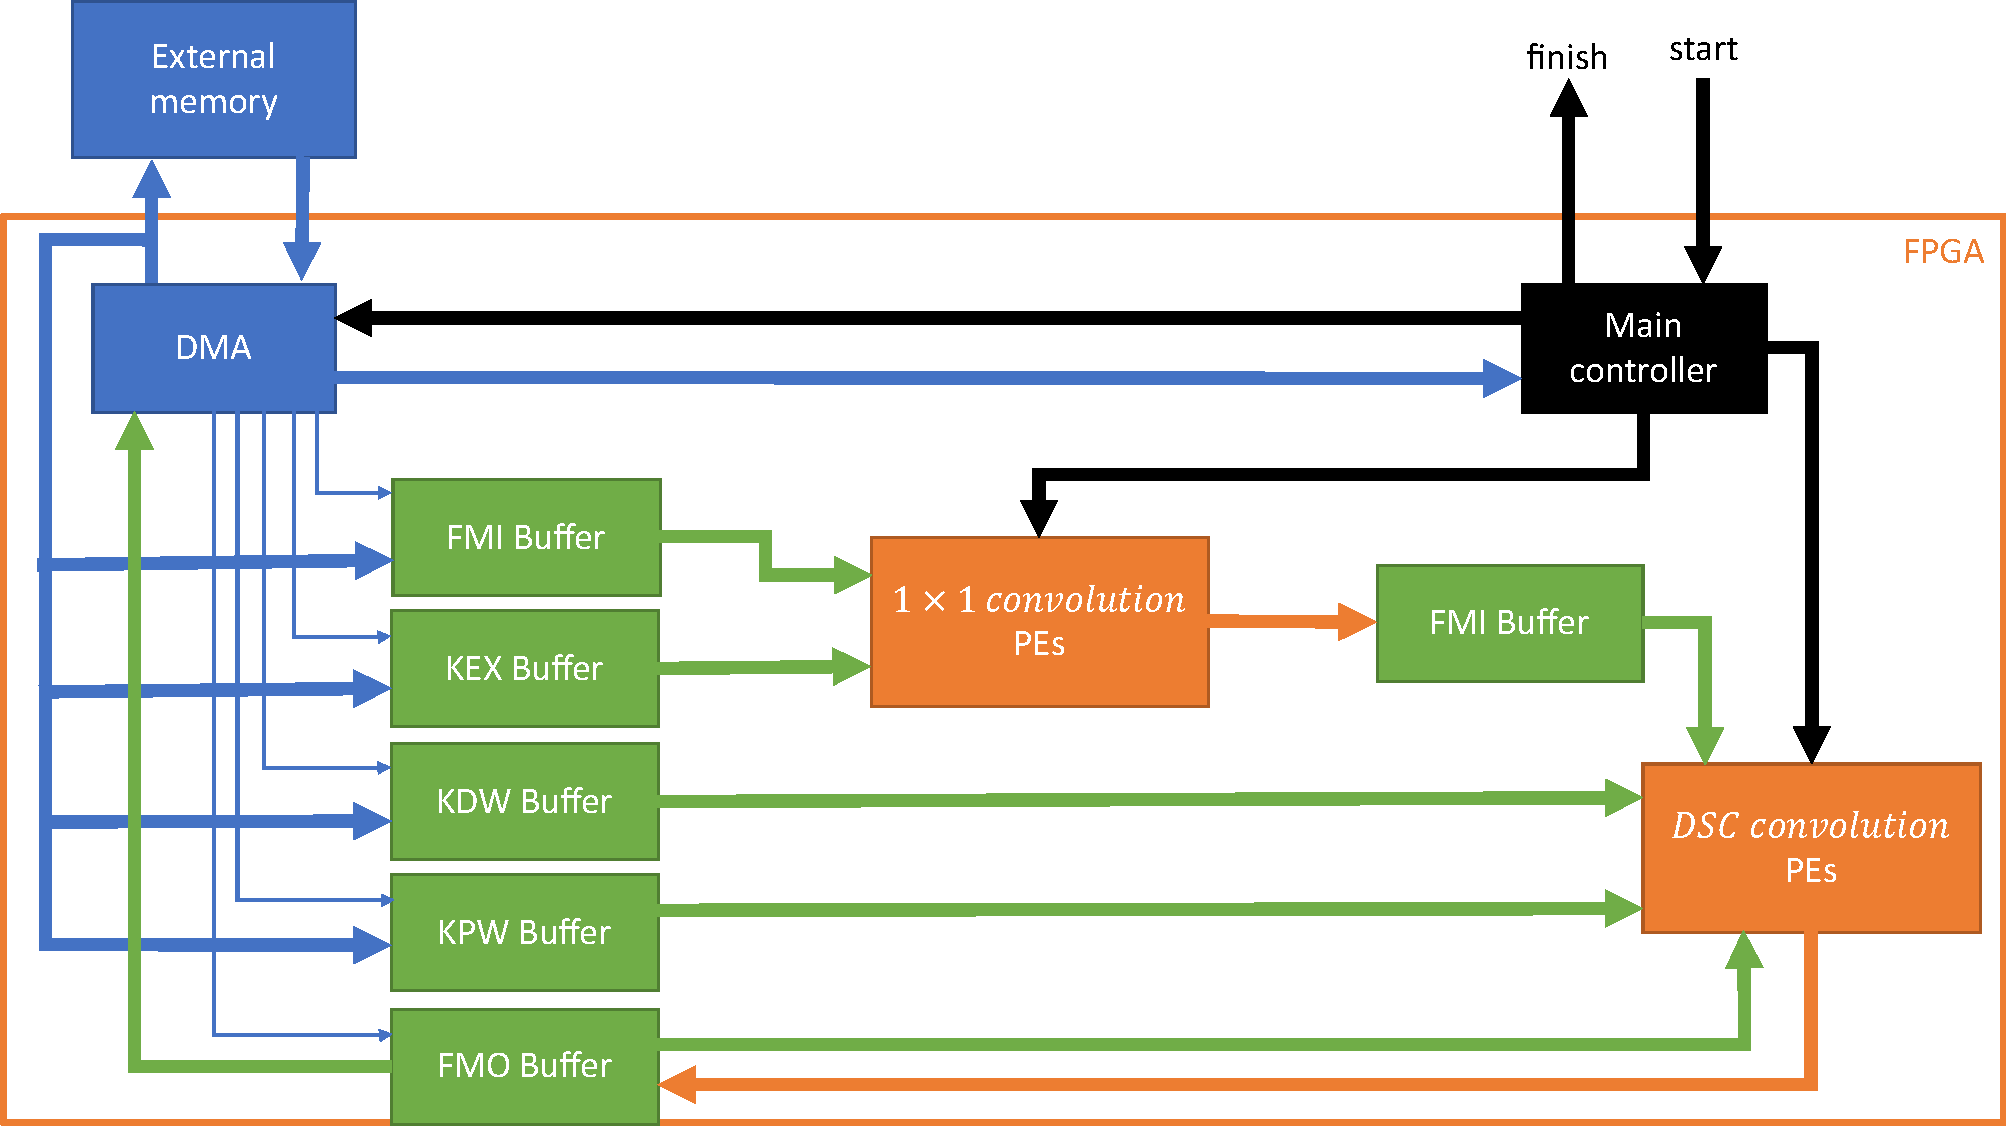
\includegraphics[width=\textwidth]{overal_archi.pdf}
    \caption{overall architecture of the accelerator}
    \label{fig:overal_archi}
\end{figure}
%

We explain more precisely the behavior of each component in the following sections. An exhaustive list of their different input and output signals can be found in Appendix \ref{appendix:sig}.
%
\subsection{External memory} \label{subs:extmem}
%
The external memory is an external component (of the \acrshort{fpga}) that contains all the data required to feed the network (MobileNetV2). Each data stored in a memory can be identified by its address (either external memory or buffer). We can identify 6 types of data:
%
\begin{enumerate}
    \item \textbf{Input \acrshort{fm}}: where the bitwidth required to represent the value of one pixel is equal to $BW_{pixel}$. Channels are stored one by one, and the content of one channel is stored line by line. For example, the memory address of the pixel at position $\left(ix, iy, if\right)$ can be expressed using Equation \eqref{eq:addr_fmi}.
    \begin{equation}
        address_{FM_{I}}(ix, iy, if) = ix + iy \times N_{ix} + if \times N_{ix} \times N_{iy}
        \label{eq:addr_fmi}
    \end{equation}
    \item \textbf{Output \acrshort{fm}}: the output \acrshort{fm} is stored in the same manner as the input \acrshort{fm}. We should add that the output \acrshort{fm} of one layer becomes the input \acrshort{fm} of the next layer. Therefore, the addresses where the output \acrshort{fm} pixels are stored become the addresses of the input \acrshort{fm} of the next layer and inversely.
    %
    \item \textbf{$1 \times 1$ kernels}: the weights of each $1 \times 1$ convolution (bottleneck layers and $1 \times 1$ convolution layers), where $BW_{weight}$ is the number of bits to represent the value of a weight and $log_2(N_{par})$ the number of bits to represent its position. Each $1 \times 1$ filter is stored kernel by kernel, and each kernel is stored weight by weight. For example, the memory address of the weight $x$ in fetching group \textquote{$group$} of kernel $f$ can be expressed using Equation \eqref{eq:addr_c11}.
    %
    \begin{equation}
        address_{K_{EX}}(kx, group, kf) = kx + group \times N_{np} + kf \times N_{np} \times N_{gr}
        \label{eq:addr_c11}
    \end{equation}
    %
    \item \textbf{Depthwise kernels}: the depthwise kernels, where the bitwidth representing one weight is equal to $BW_{weight}$. Channels are stored one by one, and the content of one channel is stored line by line. For example, the memory address of the weigth at position $\left(kx, ky, kf\right)$ can be expressed using Equation \eqref{eq:addr_dw}.
    %
    \begin{equation}
        address_{K_{DW}}(kx, ky, kf) = kx + ky \times N_{kx} + kf \times N_{kx} \times N_{ky}
        \label{eq:addr_dw}
    \end{equation}
    %
    \item \textbf{Pointwise kernels}: the kernels of the pointwise convolution. The weights are stored in the same manner as for the $1 \times 1$ filter.
    %
    \item \textbf{Standard convolution kernels}: since the first layer of MobileNetV2 is a standard convolution \cite{sandler_mobilenetv2_2018}, the weights must be also stored in the external memory, in the same manner as the depthwise filter.
\end{enumerate}

An offset for each type of data is added to the computation of the address to avoid that one address is shared between multiple data. As a result, before executing one layer, the main controller must have the following information, labelled as \textbf{Layer information}:
%
\begin{enumerate}
    \item $\boldsymbol{N_{ix}}$ and $\boldsymbol{N_{iy}}$: the spatial dimensions of the input \acrshort{fm}. Since $N_{ix}, N_{iy} \leq 224$ \cite{sandler_mobilenetv2_2018}, we can use 8 bits to represent them.
    \item $\boldsymbol{N_{if}}$ and $\boldsymbol{N_{of}}$: the number of channels of the input  and output \acrshort{fm}. Since $N_{if}, N_{of} \leq 1280$ \cite{sandler_mobilenetv2_2018}, we can use 11 bits to represent them.
    \item $\boldsymbol{t}$: the expansion factor of the $1 \times 1$ convolution. Since $t \leq 6$ \cite{sandler_mobilenetv2_2018}, we can use 3 bits to represent it.
    \item $\boldsymbol{S}$: the value of the stride. Since $S$ can be either 1 or 0 \cite{sandler_mobilenetv2_2018}, we can use 1 bit to represent it.
    \item $\boldsymbol{N_{gr}}$ and $\boldsymbol{N_{gr-int}}$: the number of fetching groups for the $1 \times 1$ convolution and the \acrshort{dsc}. Since the largest value possible for both parameters is the maximum $N_{if}$ ($N_{par} = 1$), we can use 11 bits to represent them.
    \item $\boldsymbol{Layer}$: to tell the main controller which layer is going to be executed. Since there are 4 kinds of layers in MobileNetV2 \cite{sandler_mobilenetv2_2018}, we use 2 bits to represent it. However this was not included in the design because only the bottleneck convolution was implemented.
    \item \textbf{Offsets}: the offset of the different data types must be transfered to the \acrshort{dma} in order to correctly compute the address of the required data. The number of bits required to represent one offset is the bitwidth of the address of the external memory.
\end{enumerate}
%
As a consequence, those layer information are also stored in the external memory. The overall structure of the external memory can be found in Figure \ref{fig:overal_mem}.
%
\begin{figure}[H]
    \centering
    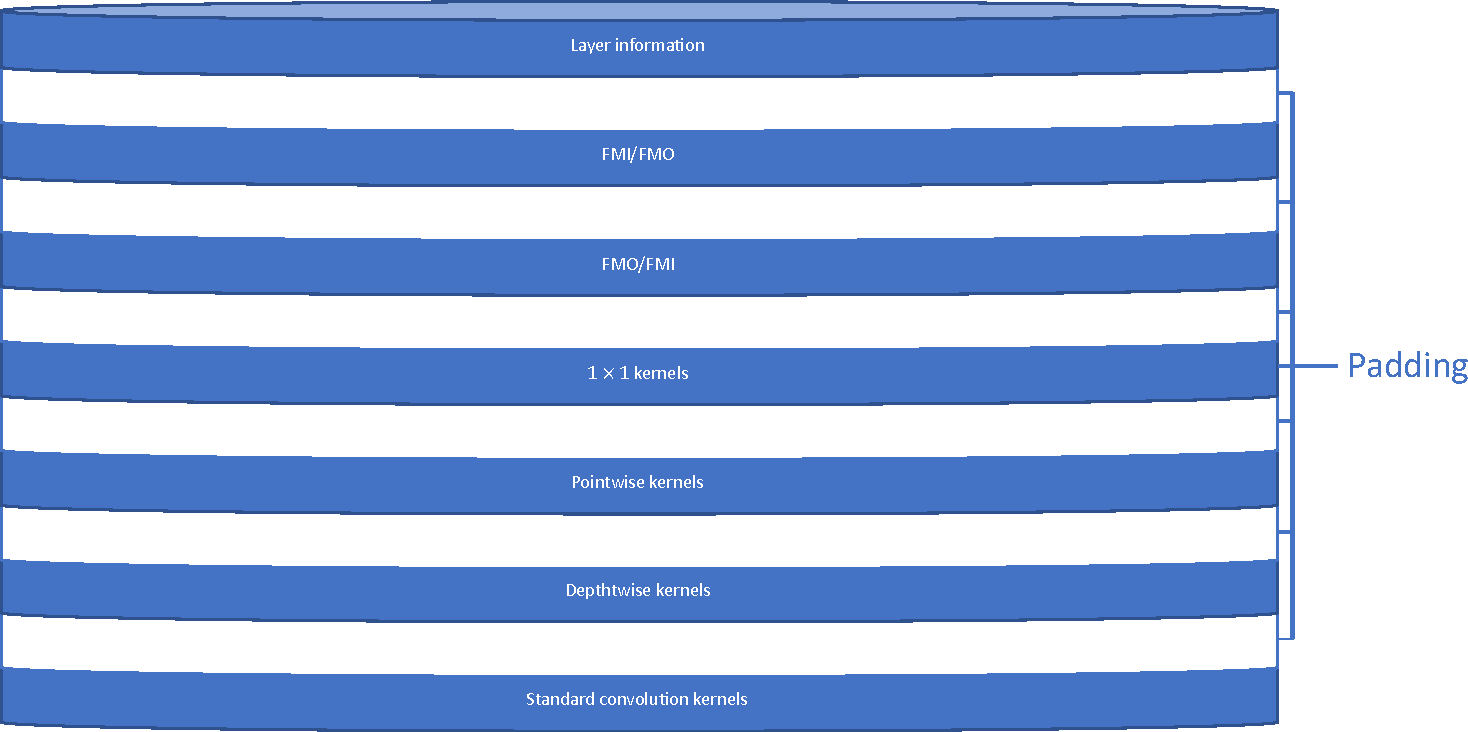
\includegraphics[width=0.75\textwidth]{overal_mem.pdf}
    \caption{overall structure of the external memory}
    \label{fig:overal_mem}
\end{figure}
%
We can now evaluate the total memory size required to hold the \acrshort{cnn}. Since this depends on the pruning parameters, we compute the upper-bound of memory required ($\alpha = 1, N_{par} = N_{if-max}$). For the same reason, we also set the memory required to store each filter or \acrshort{fm} as the memory usage of the largest element of the same type accross all layers of the network. Moreover, according to \cite{noauthor_cyclone_2018}, the maximum external memory size for Cyclone V supported is $4GB$, and hence the maximum bitwidth of the offset is $32 \ bits$. Similarly, the maximum $BW_{pixel}$ and $BW_{weight}$ is equal to $32 \ bits$.

As a result, the memory usage of the network depending on the bitwidth used to represent each pixel and weight is expressed in Equation \eqref{eq:max-extmem}.
The curve representing the maximal external memory required can be found in Figure \ref{fig:max-mem}. We can conclude that we need an external memory size of at least 70 $MB$, which is smaller than the maximal external memory of Cyclone V \acrshort{fpga} ($4 GB$)
%
\begin{align}
    \# layers_{tot} &= 21 \\
    \# layers_{standard-conv} &= 1 \\
    \# layers_{bottleneck-conv} &= 17 \\
    \# layers_{1-1-conv} &= 2 \\
    BW_{layer_{information}} &= 258 \text{ bits} \\
    Max\_FMI &= 112 \times 112 \times 32 = 401408 \\
    Max\_FMO &= Max\_FMI \\
    Max\_K11\_filter &= 320 \times 1280 = 409600 \\
    Max\_KDW\_filter &= 3 \times 3 \times 6 \times 160 = 8640\\
    Max\_KPW\_filter &= 6 \times 160 \times 320 = 307200 \\
    Max\_KSC\_filter &= 3 \times 3 \times 32 = 288
\end{align}
%
\begin{equation}
    \begin{split}
        Max\_Mem = &\left(\# layers_{tot} \times BW_{layer_{information}} \right) \\
        &+ \left( Max\_FMI \times BW_{pixel} \right) \\
        &+ \left( Max\_FMO \times BW_{pixel} \right) \\
        &+ \left( \# layers_{standard-conv} \times Max\_KSC\_filter \times BW_{weight} \right) \\
        &+ \left( \# layers_{bottleneck-conv} \times Max\_KDW\_filter \times BW_{weight} \right)\\
        &+ \left( \# layers_{bottleneck-conv} \times Max\_KPW\_filter \times \alpha \times(BW_{weight} + log_2(N_{par})) \right)\\
        &+ ( \left(\# layers_{bottleneck-conv} + \# layers_{1-1-conv}\right) \times \\
        & \ \ \alpha \times Max\_K11\_filter \times  (BW_{weight} + log_2(N_{par})) )
    \end{split}
\label{eq:max-extmem}
\end{equation}
%
\begin{figure}[H]
    \centering
    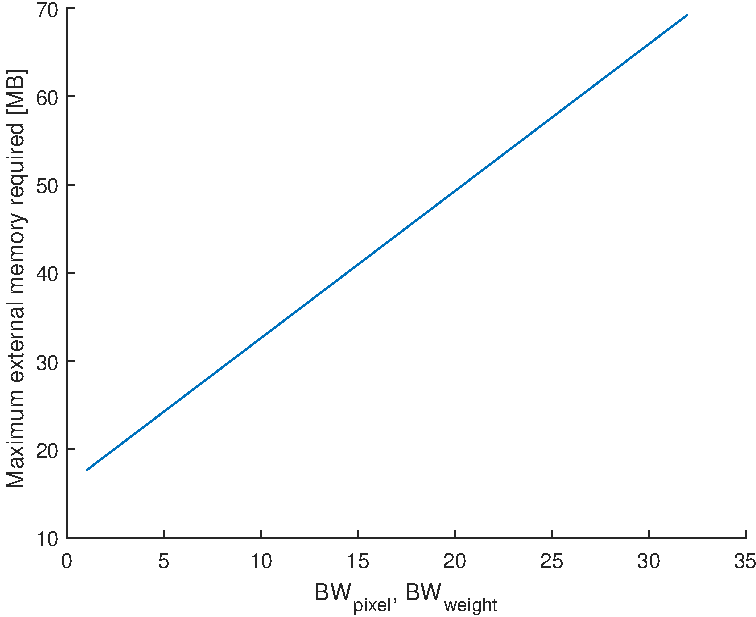
\includegraphics[width=0.75\textwidth]{maxmem.pdf}
    \caption{Maximum external memory required in $MB$ in relation with the bitwidth of each data $BW_{pixel}$ and $BW_{weight}$}
    \label{fig:max-mem}
\end{figure}
%
The maximum memory required can be reduced with pruning. For example, by modifying Equation \eqref{eq:max-extmem}, with $N_{par} = 8, N_{np} = 4$, and $BW_{weight} = BW_{pixel} = 16$, the total memory required is equal to 16.54 $MB$.
%
\subsection{Main controller}
%
The role of the main controller is to synchronize the different components of the architecture (except the memory components). Therefore, each component is a \textquote{slave} that stays in an idle state until the main controller wakes up one of them to perform a particular operation.

To wake up a component, the main controller sends it a starting signal $s_{*}$ and optionnaly additional information about the operation to perform. Afterwards, the main controller remains idle, waiting for the component to terminate its operation. Once the component has completed its task, it sends a finishing signal $f_{*}$ to the main controller.

The main controller remains in an idle state until it receives a starting signal indicating that the external memory contains all data to perform a bottleneck convolution. I have implemented the main controller to compute one bottleneck convolution, but its architecture could be extended to iterate through all the layers of the network.

%
\begin{figure}
    \centering
    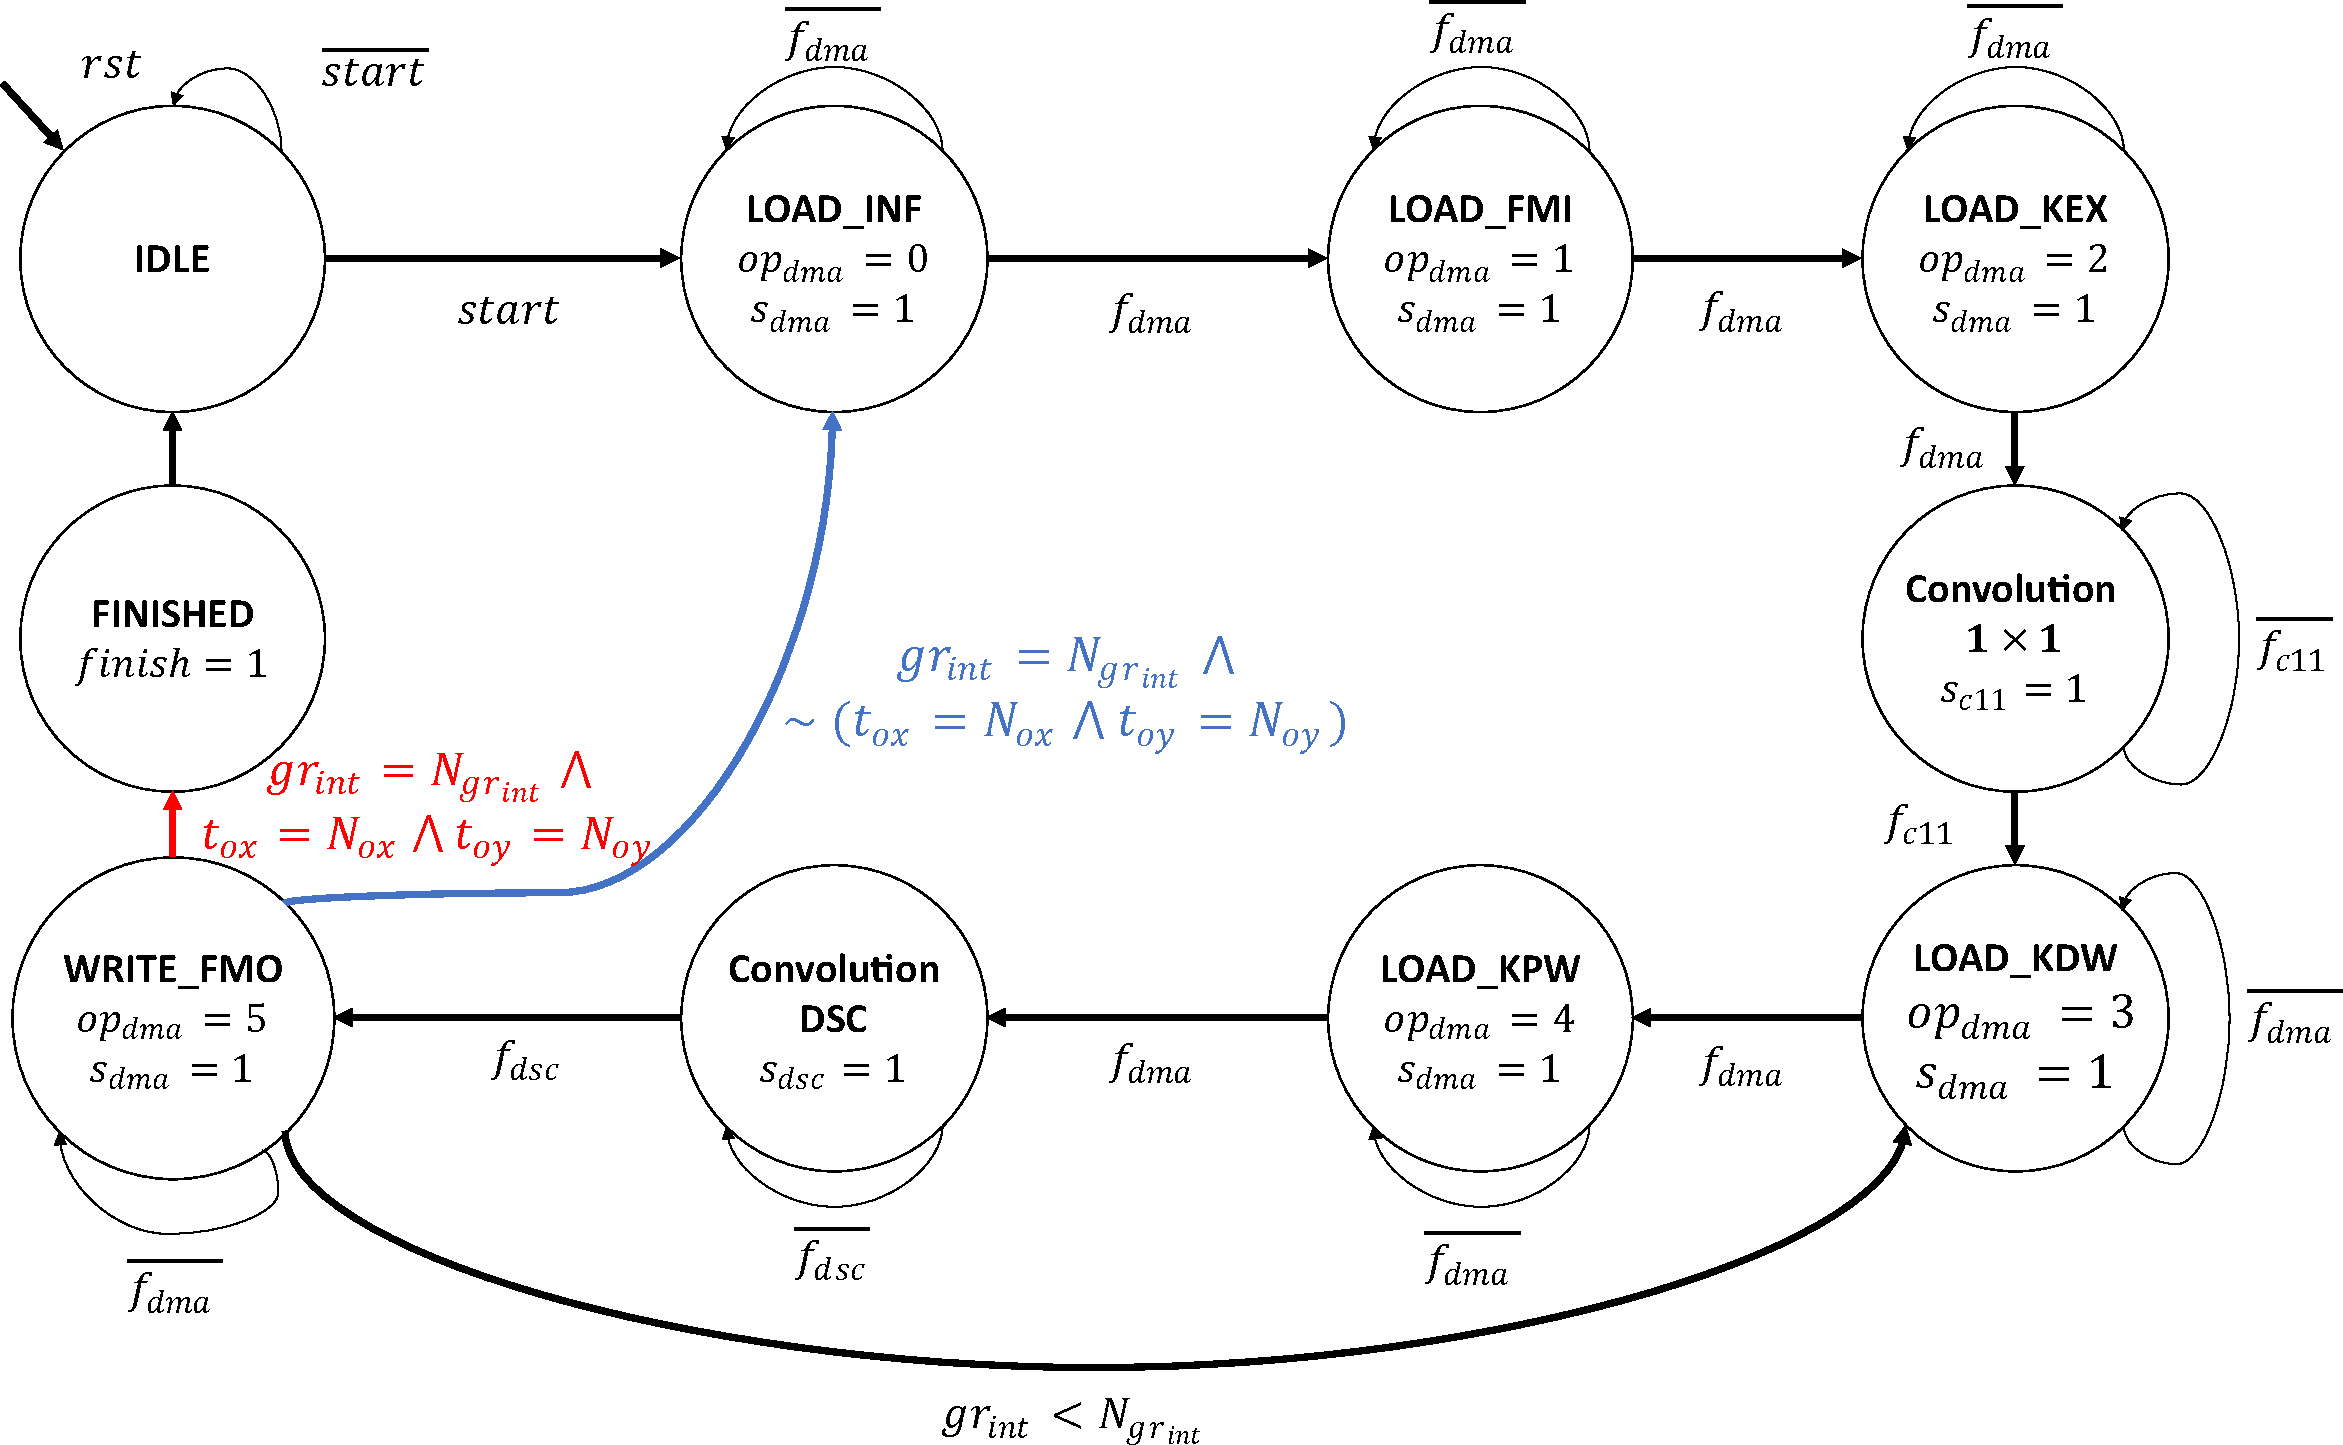
\includegraphics[width=\textwidth]{fsm-mc.pdf}
    \caption{\acrshort{fsm} of the main controller}
    \label{fig:fsm_mc}
\end{figure}
We can describe the behavior of the main controller using a \acrfull{fsm}, as illustrated in Figure \ref{fig:fsm_mc}. For the sake of clarity, additional informations transmitted to the components are not shown in the Figure. The \textbf{IDLE} state is the state where the main controller is waiting to perform a bottleneck convolution. Once the main controller has received a starting signal, it performs the following operations:
%
\begin{figure}
    \centering
    %
    \begin{subfigure}[t]{.49\textwidth}
        \centering
        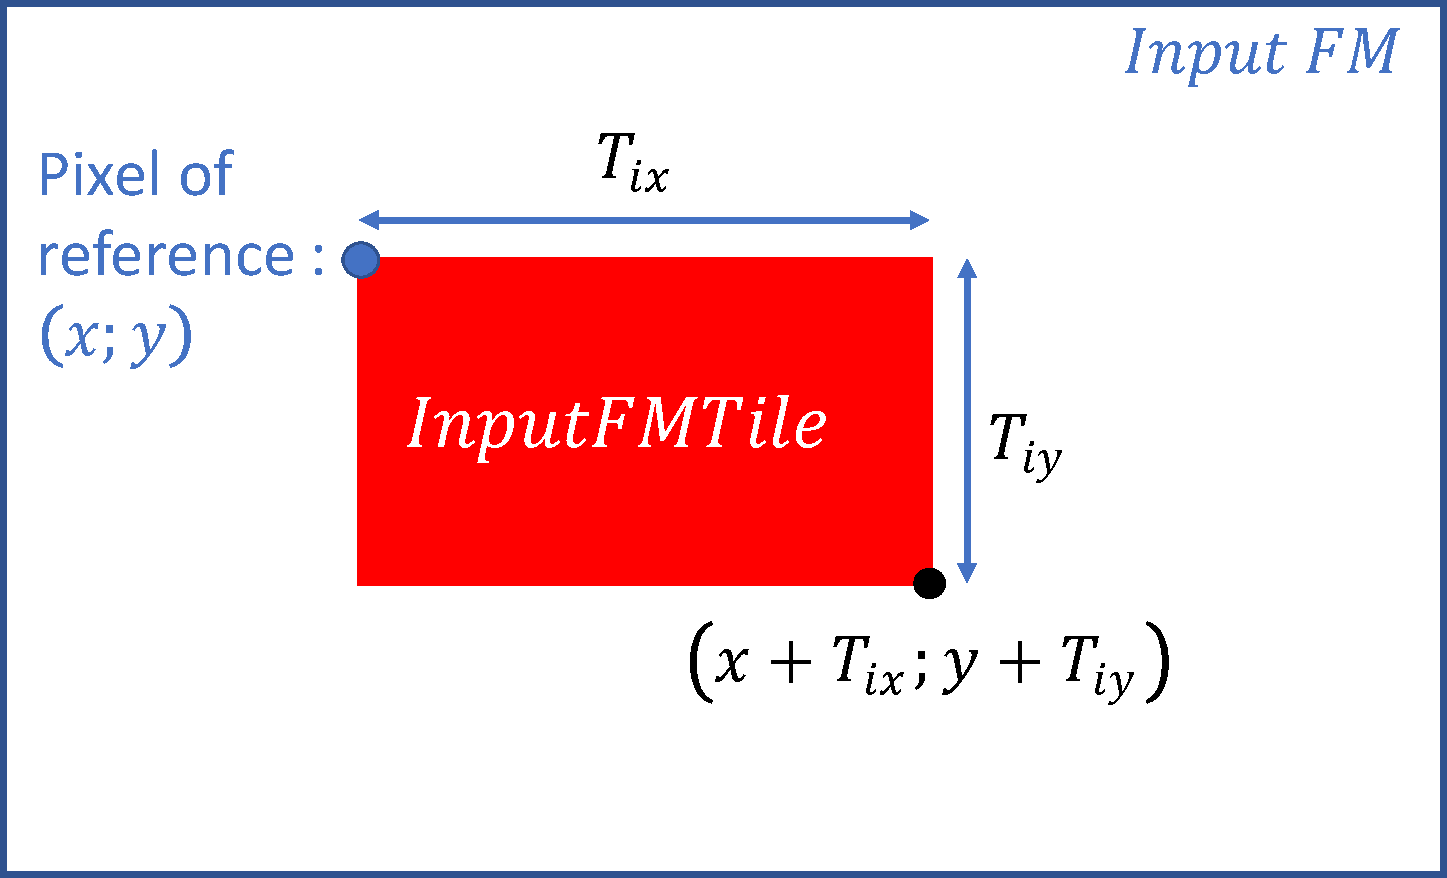
\includegraphics[width=\linewidth]{pixofref.pdf}
        \caption{Example of pixel of reference for an input \acrshort{fm} tile}
        \label{fig:pix_of_ref}
    \end{subfigure}
    %
    \begin{subfigure}[t]{.49\textwidth}
        \centering
        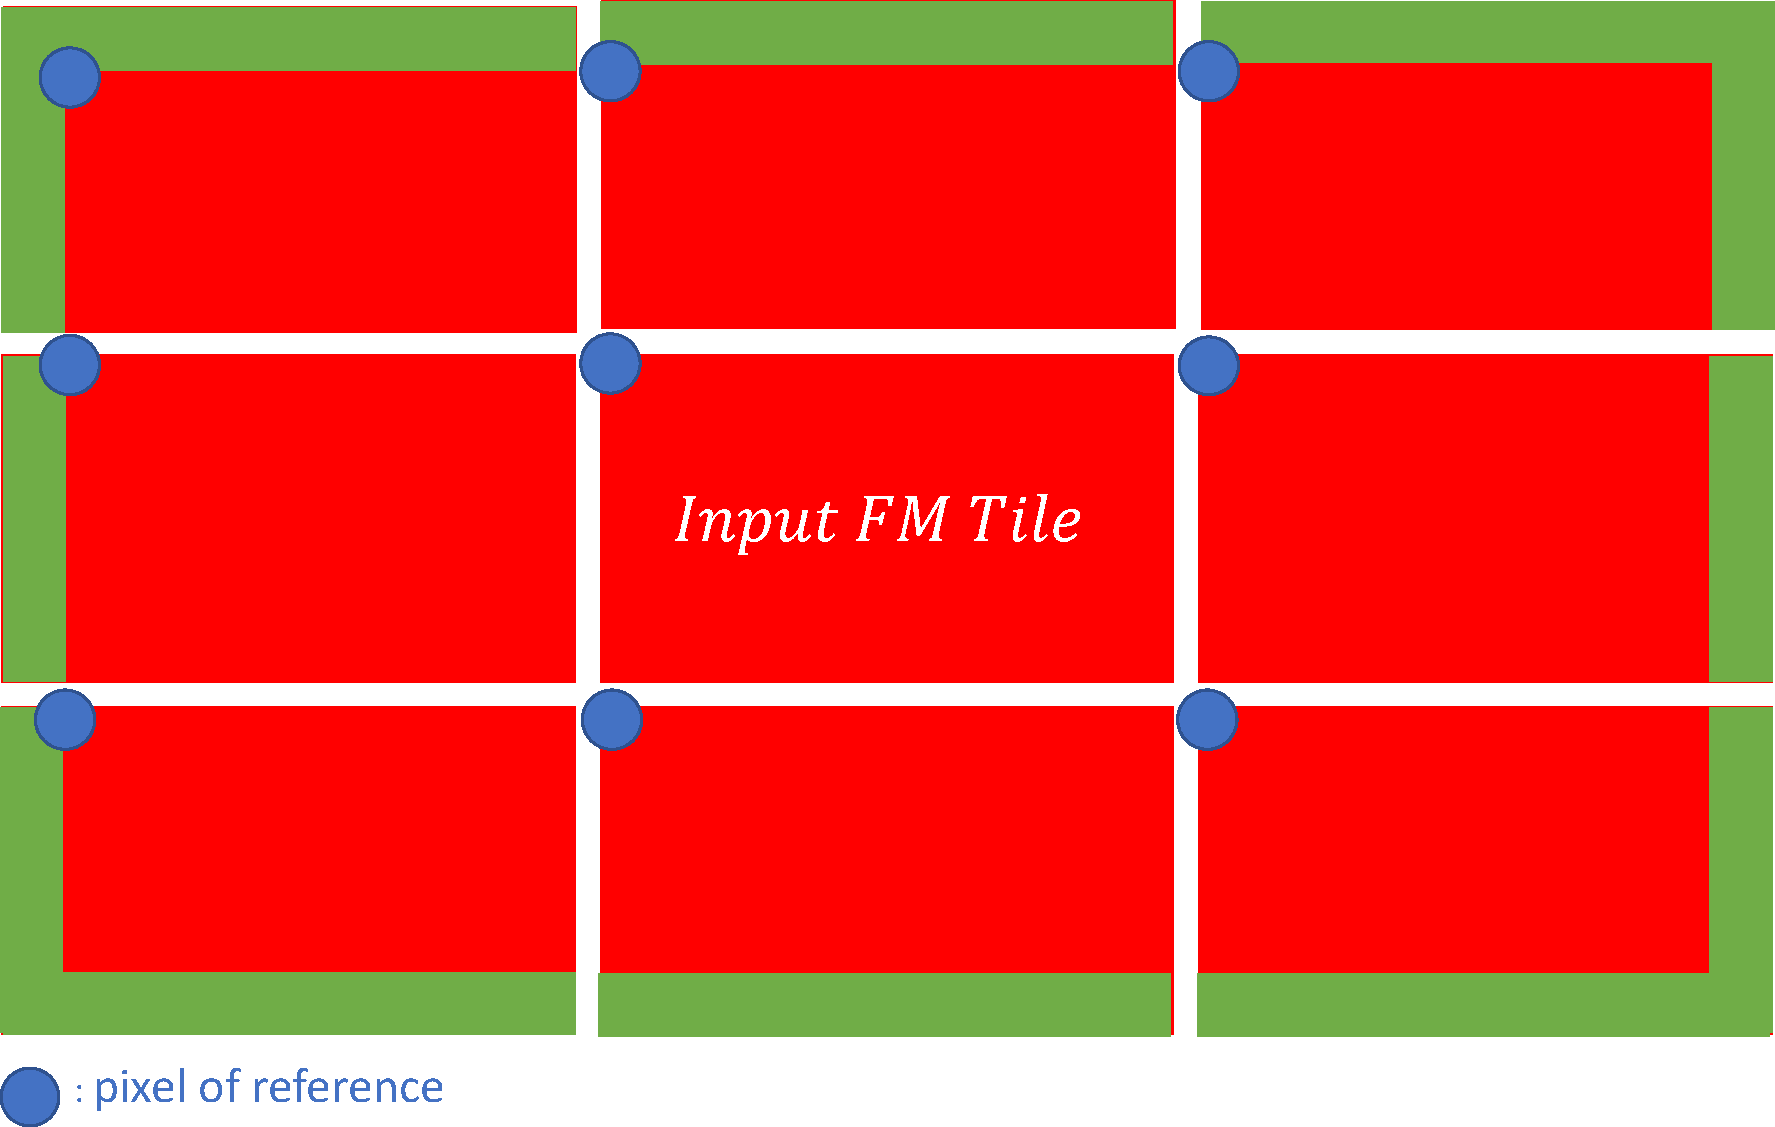
\includegraphics[width=\linewidth]{tilepadding.pdf}
        \caption{Padding configuration of input \acrshort{fm} tiles, where red area represent pixels fetched from external memory and green area represent padding pixels}
        \label{fig:tile_padding}
    \end{subfigure}
    %
    \caption{Illustration of the concept of pixel of reference and padding}
\end{figure}
%
\begin{enumerate}
    \item \textbf{LOAD\_INF}: to perform the bottleneck convolution, the main controller first needs to fetch the layer information stored in the external memory. Therefore it tells the \acrshort{dma} to fetch them ($op_{dma} = 0$).
    %
    \item \textbf{LOAD\_FMI}: the bottleneck convolution starts by fetching a tile of inputs and weights from the main memory. As all inputs in the channel-axis are buffered (corresponding to all the fetching groups), an input \acrshort{fm} tile can be determined only by the spatial coordinates of the tile first element - pixel of reference (with the smallest $(x, y)$). Indeed, the \acrshort{dma} can fetch, for each channel, all pixels in the range $[(x, y); (x+T_{ix}, y+T_{iy})]$, which corresponds to the tile, as illustrated in Figure \ref{fig:pix_of_ref}.
    As a result, when the main controller asks the \acrshort{dma} to load into the on-chip memory a tile of input \acrshort{fm} ($op_{dma} = 1$), it also transfers the spatial coordinates and the memory address of its pixel of reference. Moreover, since we have to add padding to the tile (spatial dimensions are not reduced by the convolution operations), 0 value pixels are stored in the on-chip memory at corresponding positions when the reference pixel is on one edge of the input \acrshort{fm}, as shown in Figure \ref{fig:tile_padding}.
    %
    \item \textbf{LOAD\_KEX}: after fetching the input \acrshort{fm} tile, the main controller asks the \acrshort{dma} to load the $N_{par}$ $1 \times 1$ kernels into the on-chip memory ($op_{dma} = 2$), corresponding to the intermediate fetching group $group_{int}$. %Rajouter le channel de ref
    \item \textbf{CONV\_11}: after loading the weights and pixels, the $1 \times 1$ convolution can be performed. Once the $N_{par}$ intermediate channels corresponding to the intermediate fetching group $group_{int}$ have been produced, the \acrshort{dsc} can be executed.
    \item \textbf{LOAD\_KDW} and \textbf{LOAD\_KPW}: before doing the \acrshort{dsc}, the pointwise and depthwise kernels corresponding to the intermediate fetching group should be loaded by the \acrshort{dma} ($op_{dma} = 3$ and $op_{dma} = 4$).
    \item \textbf{CONV\_DSC}: all output \acrshort{fm} tile partial products can be computed by performing the \acrshort{dsc} on the $N_{par}$ intermediate channels. If all intermediate fetching groups have been processed, final results are computed and can be written into the external memory. Otherwise, the next $N_{par}$ intermediate channels should be computed. Moreover, since output \acrshort{fm} partial results will be kept in on-chip memory, the main controller indicates to the \acrshort{dsc} \acrshort{pe}s whether the values read from the \textit{FMO Buffer} should be consired as valid. If it is not the case, the value should be set to 0.
    \item \textbf{WRITE\_FMO}: this state indicates that there are only final results in the \textit{FMO Buffer}. The main controller tells the \acrshort{dma} that its content can be written to the external memory ($op_{dma} = 5$). As for the input \acrshort{fm} tiles, the output \acrshort{fm} tiles are determined by their pixel of reference, which is also transmitted to the \acrshort{dma}. If all tiles have been processed, the bottleneck convolution is completed and the main controller state turns to \textbf{FINISHED}. Otherwise, a new tile has to be processed and main controller returns to \textbf{LOAD\_FMI} state.
    \item \textbf{FINISHED}: The bottleneck convolution is done and the main controller sets the finish signal.
\end{enumerate}
%
\subsection{DMA}
%
The purpose of the \acrshort{dma} is to fill the \textbf{data buffer} with its corresponding tile fetched from external memory and write the output pixels into the external memory. Therefore, it has to manage six types of operation, referenced by its operation number $op_{dma}$:
%
\begin{itemize}
    \item $op_{dma} = 0$: Load the layer information
    \item $op_{dma} = 1$: Load an input \acrshort{fm} tile, referenced by its pixel of reference. The \acrshort{dma} needs as extra information the coordinate and the memory address of that pixel of reference.
    \item $op_{dma} = 2$: Load the $1 \times 1$ kernels used to produce the intermediate fetching group $group_{int}$ of size $N_{par}$. The \acrshort{dma} needs as extra information the first kernel and the memory address of its first weight to correctly load the $N_{par}$ kernels.
    \item $op_{dma} = 3$: Load the depthwise kernels corresponding to the intermediate fetching group $group_{int}$ of size $N_{par}$. The \acrshort{dma} needs as extra information the first kernel of the group and the memory address of its first weight to correctly load the $N_{par}$ kernels.
    \item $op_{dma} = 4$: Load the weight fetching group (of size $N_{np}$) of all pointwise kernels corresponding to the intermediate fetching group $group_{int}$. The \acrshort{dma} needs as extra information the position of the first weight in the fetching group and its memory address.
    \item $op_{dma} = 5$: Write the content of the \textbf{FMO Buffer} into the external memory, which corresponds to a tile of output \acrshort{fm}. As this tile is referenced by its pixel of reference, the \acrshort{dma} needs as extra information the coordinate and the memory address of that pixel of reference.
\end{itemize}

%
\begin{figure}
    \centering
    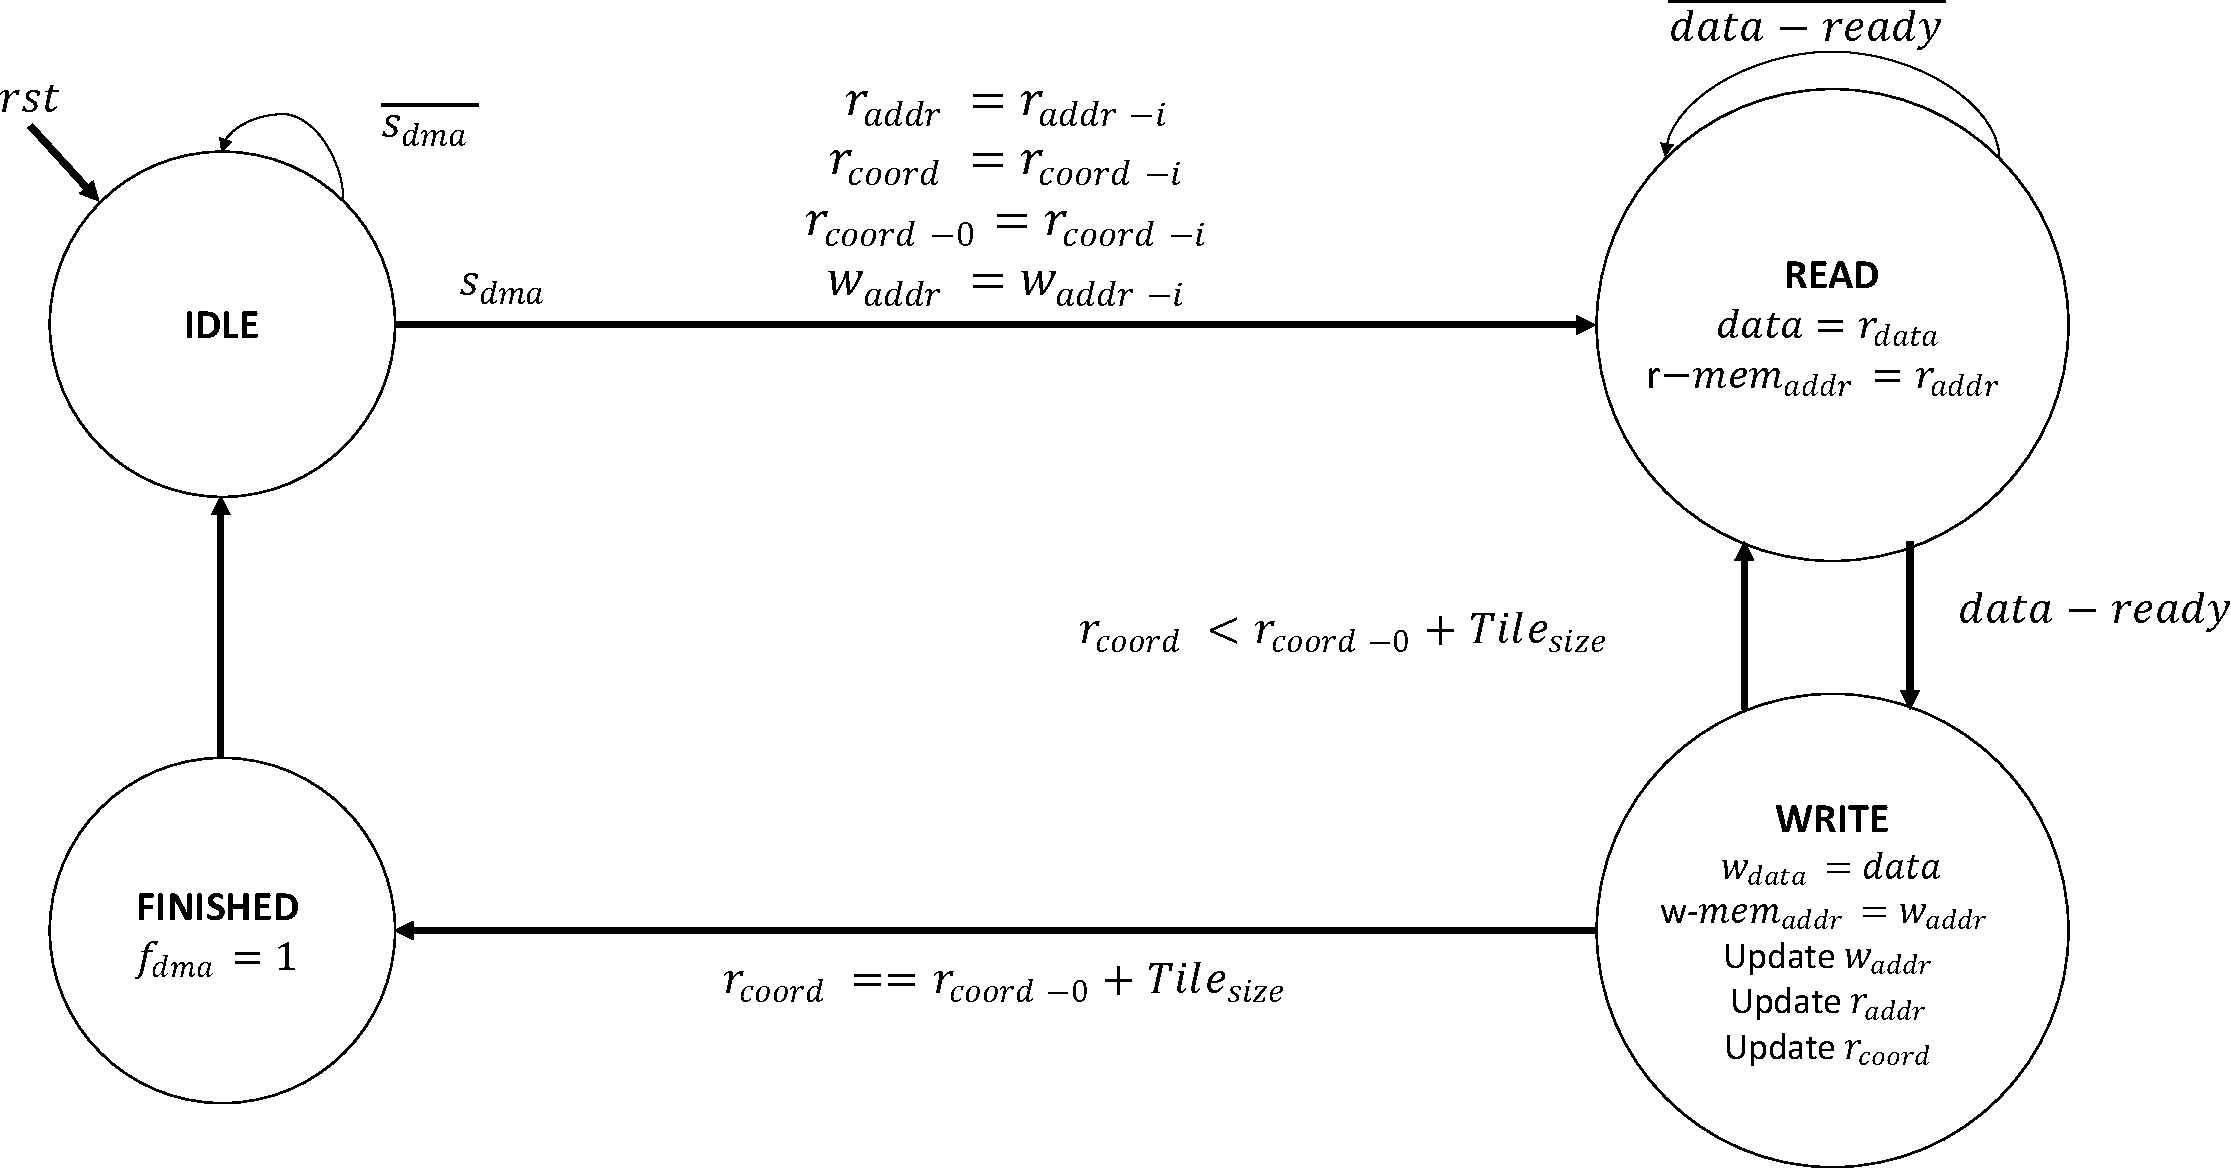
\includegraphics[width=\textwidth]{fsm-dma.pdf}
    \caption{\acrshort{fsm} of the \acrshort{dma}}
    \label{fig:fsm_dma}
\end{figure}
When the main controller asks the \acrshort{dma} for a transfer, it sets its start signal, which operation to execute ($op_{dma}$), and all extra information related to the external memory required. If the \acrshort{dma} reads or writes into a buffer, the initial address $r_{addr-i}/w_{addr-i}$ can be set to 0. Indeed, buffer addresses start from 0 to $Buffer_{N_{elem}} - 1$. The behavior of the \acrshort{dma} can be expressed using a \acrshort{fsm}, as found in Figure \ref{fig:fsm_dma}. A general \acrshort{fsm} has been illustrated because each operation shares the same structure. As the \acrshort{dma} only fetches data from one memory and writes the data into another one, each operation is composed of 2 states:
\begin{itemize}
    \item \textbf{READ}: the \acrshort{dma} fetches the required data at a address $r_{addr}$. Once the data is loaded by the \acrshort{dma}, it moves to the next state to write the data in the on-chip memory. When loading the input \acrshort{fm} tile, if the address corresponds to a padding pixel, the value to write is 0 and the \acrshort{dma} directly moves to the \textbf{WRITE} state. If the data is fetched from the external memory, the \acrshort{dma} sets the read request signal $r_{request_{extmem}}$ (enabling a transfet) waits the data read from the external memory to be valid ($r_{valid_{extmem}}$). But if the data is fetched from a buffer, the process can be pipelined. That is why, before the \acrshort{dma} reads data from the on-chip memory, it is in a state called \textbf{RAM\_LOADING} to initialize the pipeline process.
    \item \textbf{WRITE}: the \acrshort{dma} sends a write signal and the associated data $w_data$ and address $w_{address}$ to the corresponding memory . If the operation is finished (the tile has been fetches), the \acrshort{dma} goes into the \textbf{FINISHED} state. Otherwise, it updates the address of the next data to fetch and goes back to the \textbf{READ} state.
\end{itemize}

The \acrshort{dma} has therefore signals for reading $r_{extmem}$ a data at address $address_{extmem}$. Since the \acrshort{dma} performs one transfer at a time, we can share the fetched data (to be written) $w_{data}$ between all memory component and we set the write signal to the corresponding component. In a similar way, the signal to access or write data in a buffer $ram_{addr}$ can also be shared between the different buffers. As the \acrshort{dma} reads the contrent of only one buffer, we define the corresponding signal as $r_{ram}$ (and hence at address $ram_{addr}$).
%
\subsection{1\texttimes1 convolution PE}
%
\begin{figure}
    \centering
    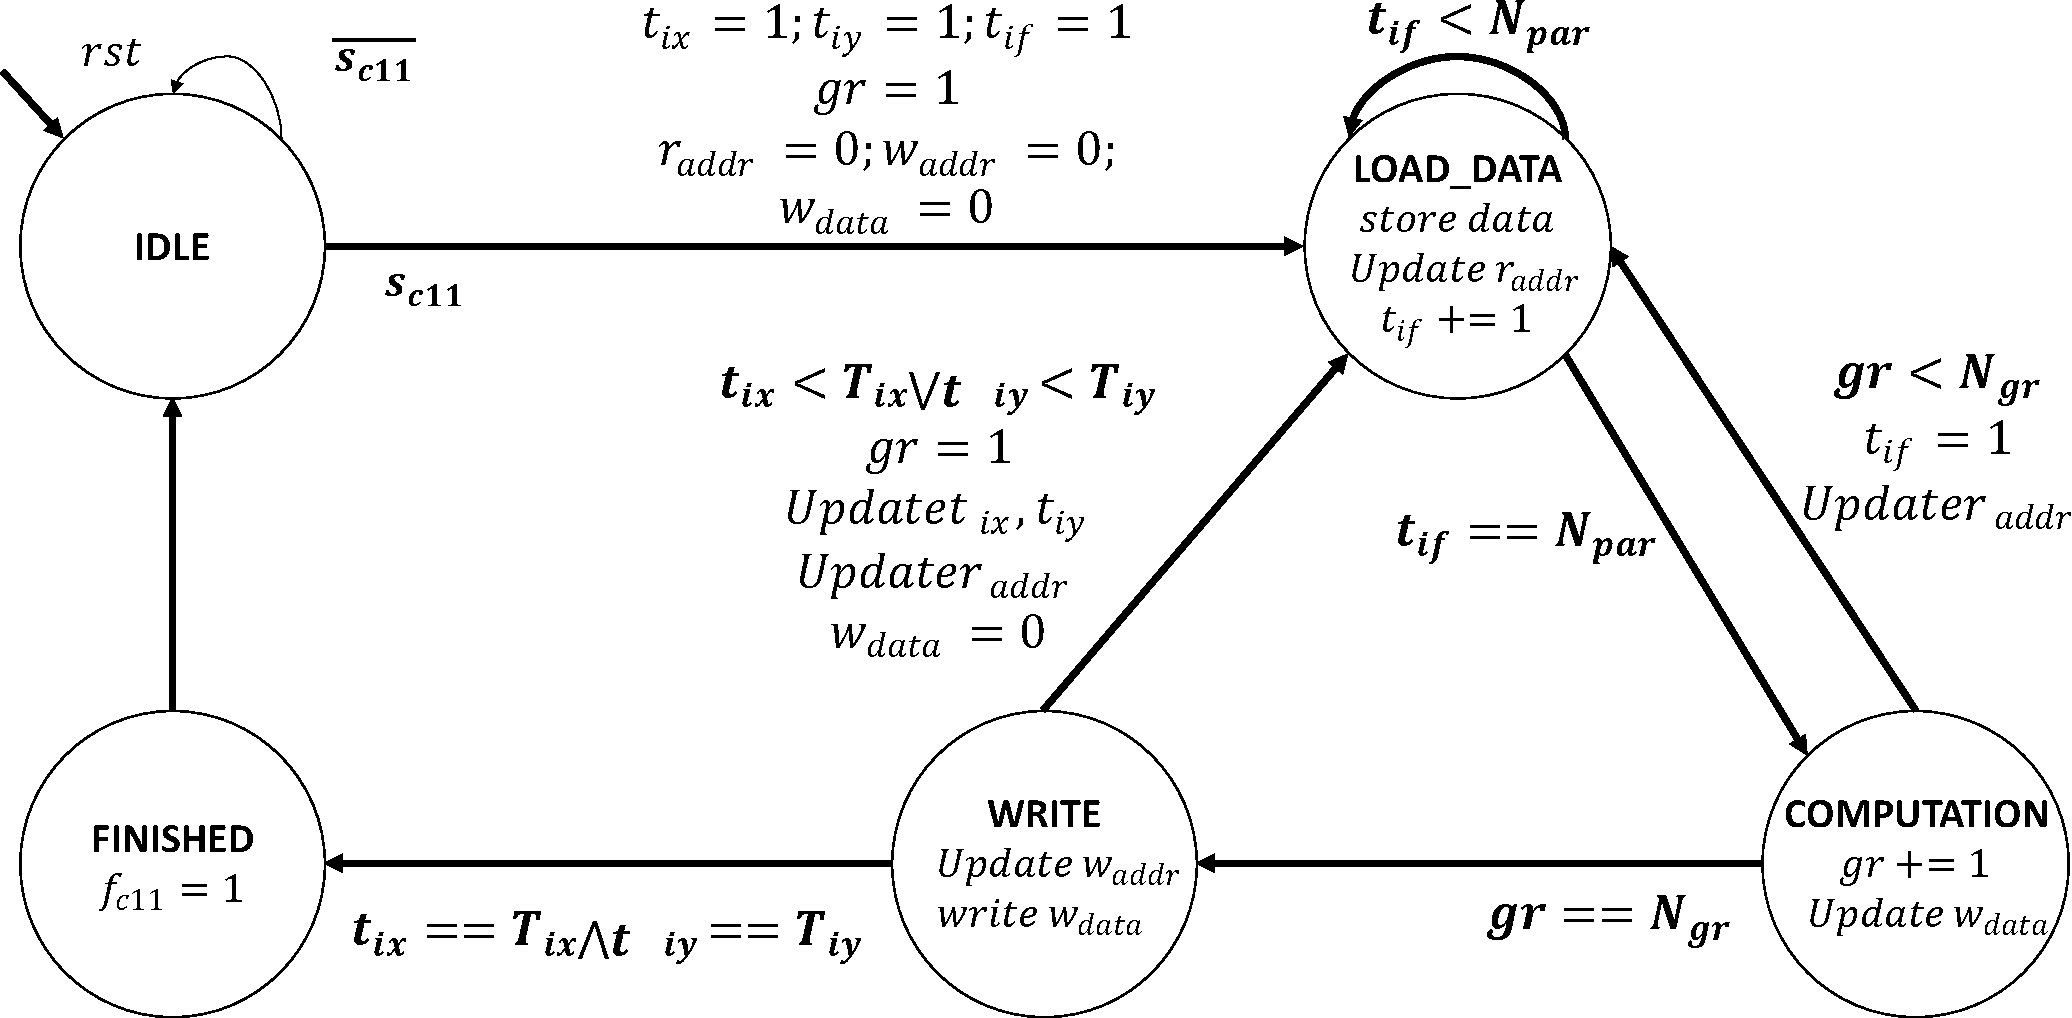
\includegraphics[width=\textwidth]{fsm-c11.pdf}
    \caption{\acrshort{fsm} of the 1\texttimes1 convolution PE}
    \label{fig:fsm_c11}
\end{figure}
%
The purpose of this component is to execute the Algorithm \ref{pseudocode:c11}. The behavior of the \acrshort{pe} can be expressed using a \acrshort{fsm}, as found in Figure \ref{fig:fsm_c11}.

\begin{figure}
    \centering
    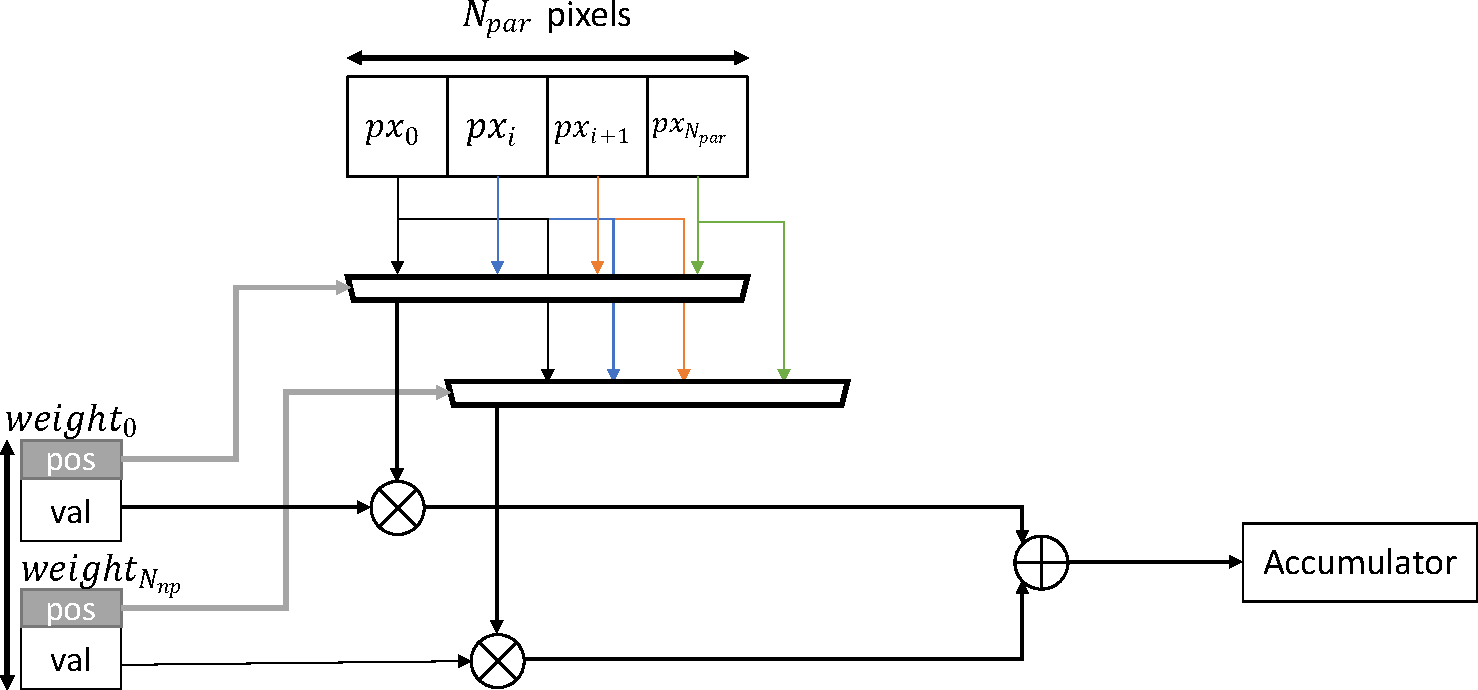
\includegraphics[width=\linewidth]{hardware_conv11.pdf}
    \caption{\acrshort{pe} structure performing the convolution where $N_{par} = 4$ and $N_{np} = 2$, inspired by \cite{kang_accelerator-aware_2020}}
    \label{fig:c11_hardware}
\end{figure}
%
When the \acrshort{pe} receives a starting signal, it means that the \textbf{FMI} and \textbf{KEX BUFFERS} contain the data to execute the next $1 \times 1$ convolution. For each fetching group corresponding to an intermediate pixel at address $w_{addr}$, the \acrshort{pe} loads the corresponding $N_{par}$ inputs and $N_{np}$ weights into its registers (\textbf{LOAD\_DATA} state).
Once it is done, the computation can be performed (\textbf{COMPUTATION} state). Since the convolution is fully-unrolled, we can use the \acrshort{pe} structure from \textcite{kang_accelerator-aware_2020}, which is shown in Figure \ref{fig:c11_hardware}. The output result is then summed with the content of the accumulator (which contains 0 for the first fetching group).

When the convolution is done for one intermediate pixel, the result is fed to the ReLU6 activation (see Section \ref{subs:acti}), and its output is written into the \textbf{FMINT BUFFER}. If all pixels required for the \acrshort{dsc} have been computed, the \acrshort{pe} sends an ending signal to the main controller (\textbf{FINISHED} state). Otherwise it computes the next intermediate pixel.

This \acrshort{pe} is described for the its use in the bottleneck convolution, but is could also be used in the $1 \times 1$ layers.
%
\subsection{DSC PE}
%
\begin{figure}
    \centering
    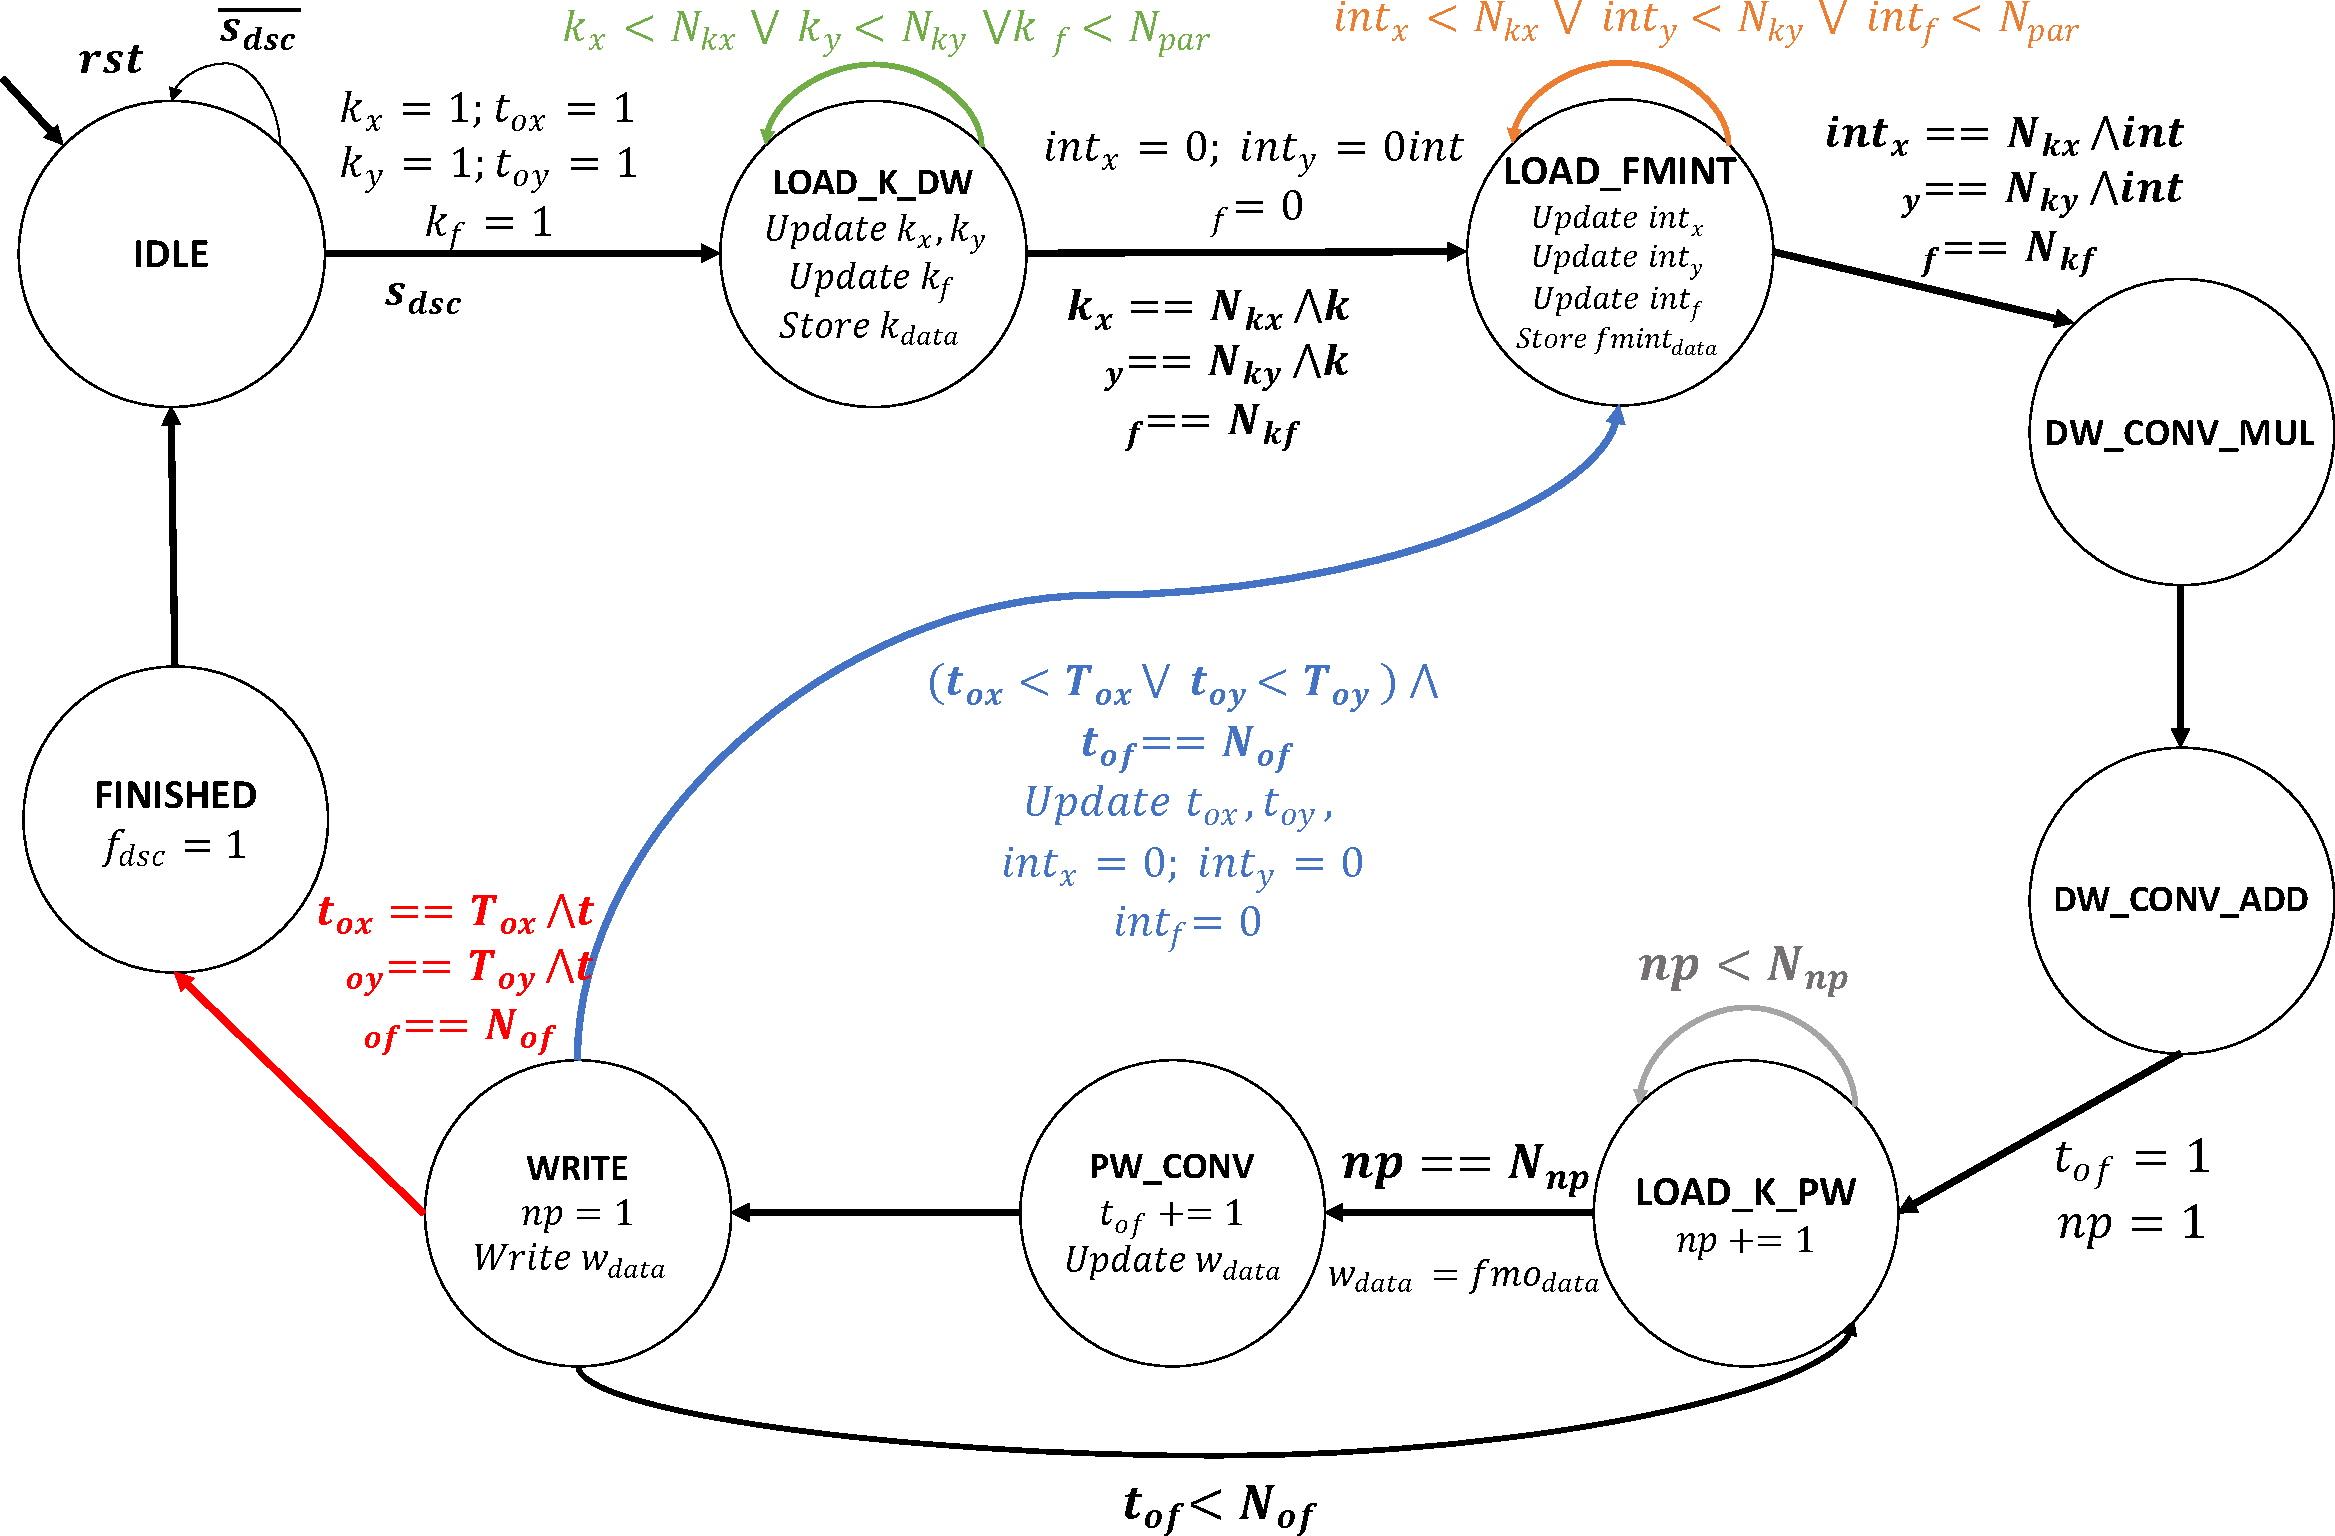
\includegraphics[width=\textwidth]{fsm-dsc.pdf}
    \caption{\acrshort{fsm} of the \acrshort{dsc} \acrshort{pe}}
    \label{fig:fsm_dsc}
\end{figure}
This \acrshort{pe} is designed to perform the \acrshort{dsc}. Once the $1 \times 1$ convolution has computed the next intermediate fetching group and the \textbf{Buffers} containts the required data, we can do the \acrshort{dsc} as in Algorithm \ref{pseudocode:dsc}. The \acrshort{pe} can be described as a \acrshort{fsm} executing the proposed algorithm in Figure \ref{fig:fsm_dsc}.

\begin{figure}
    \centering
    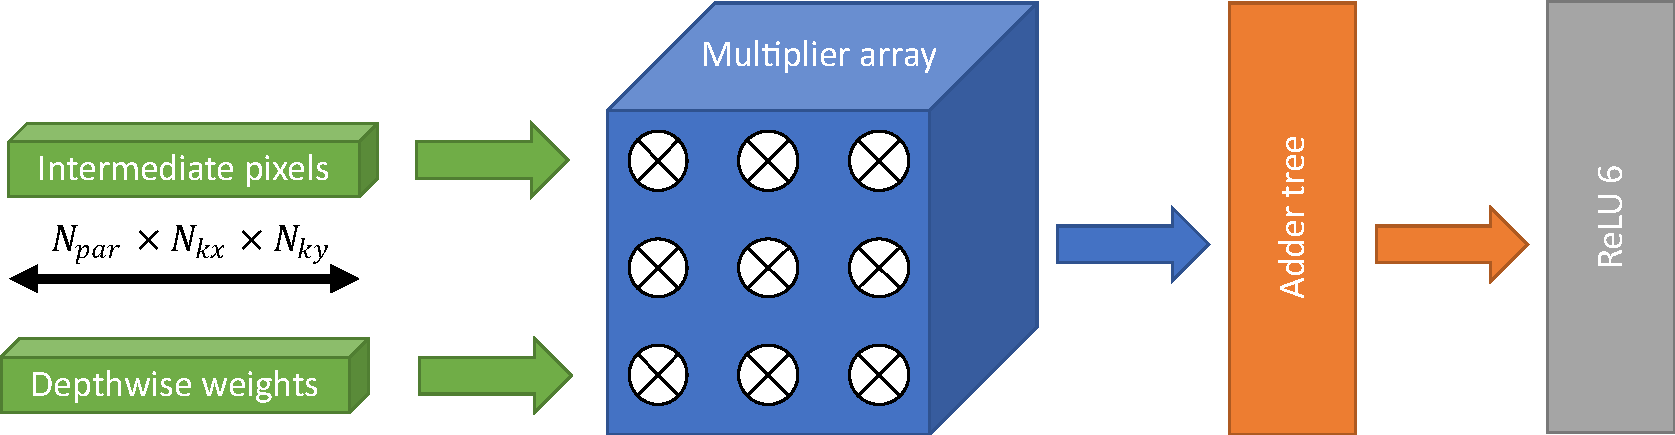
\includegraphics[width=\textwidth]{hardware-dw.pdf}
    \caption{\acrshort{pe} structure performing the depthwise convolution, inspired by \cite{bai_cnn_2018}}
    \label{fig:dsc_hardware}
\end{figure}
%
The \acrshort{pe} has the same structure as the 1\texttimes1 convolution PE. However, the 2 \acrshort{pe}s diverges on the following elements:
\begin{itemize}
    \item For each intermediate pixels, the 1\texttimes1 \acrshort{pe} performs $N_{gr}$ $1 \times 1$ partial convolutions on the input pixels and $1 \times 1$ kernels directly fetched from the buffers.
    %
    \item On the other hand, for the \acrshort{dsc} \acrshort{pe} must first loads the $N_{kx} \times N_{ky} \times N_{par}$ intermediate pixels and depthwise weights (\textbf{LOAD\_K\_DW} and \textbf{LOAD\_FMINT} states). This is done in two different states because the depthwise is fully-unrolled and therefore we keep all required weights into the registers. We have to only fetch them once from the external memory.
    %
    \item After it has loaded the input pixels and the depthwise weights, the depthwise convolution can be performed. To execute the depthwise convolution for each intermediate channels, we can use the same \acrshort{pe} as \textcite{bai_cnn_2018}, as illustrated in Figure \ref{fig:dsc_hardware}. First we do a element-wise multiplication using a multiplier array between pixels and weights (\textbf{DW\_CONV\_MUL} state). Then, we simply have to sum the products belonging to the same channel to obtain the $N_{par}$ depthwise produtcs used as input for the pointwise convolution (\textbf{DW\_CONV\_ADD} state). Then the registers store the results of the ReLU6 activation function for the \acrshort{dsc}.
    %
    \item We can perform the partial \acrshort{dsc} for the $N_{of}$ channels of spatial coordinate $o_x, o_y$. For each channel, we load the $N_{np}$ weights corresponding to that channel and the intermediate fetching group (\textbf{LOAD\_K\_PW} state). We also load the partial sum stored in the \textbf{FMO Buffer} to sum it with the results of the convolution (\textbf{PW\_CONV} state). However, if it is the first intermediate fetching group, this value is set to 0 ($first\_par\_i$ signal, set by the main controller).
    The structure of the \acrshort{pe} performing the pointwise convolution is the same as Figure \ref{fig:c11_hardware}. Then the sum between the partial sum stored and the result of the convolution is stored in the \textbf{FMO Buffer} (\textbf{WRITE} state).
    %
    \item When all the partial sum have been produced, the \acrshort{pe} moves to the \textbf{FINISHED} state and sets its finishing signal.
\end{itemize}

The \acrshort{dsc} \acrshort{pe} could be extended to support the standard, as pointed out by \textcite{bai_cnn_2018}. Indeed, if we consider sum all products in the multiplier array instead of only those belonging to the same channel, we perform the standard convolution.
%
\subsection{Buffer}
%
\begin{figure}
    \centering
    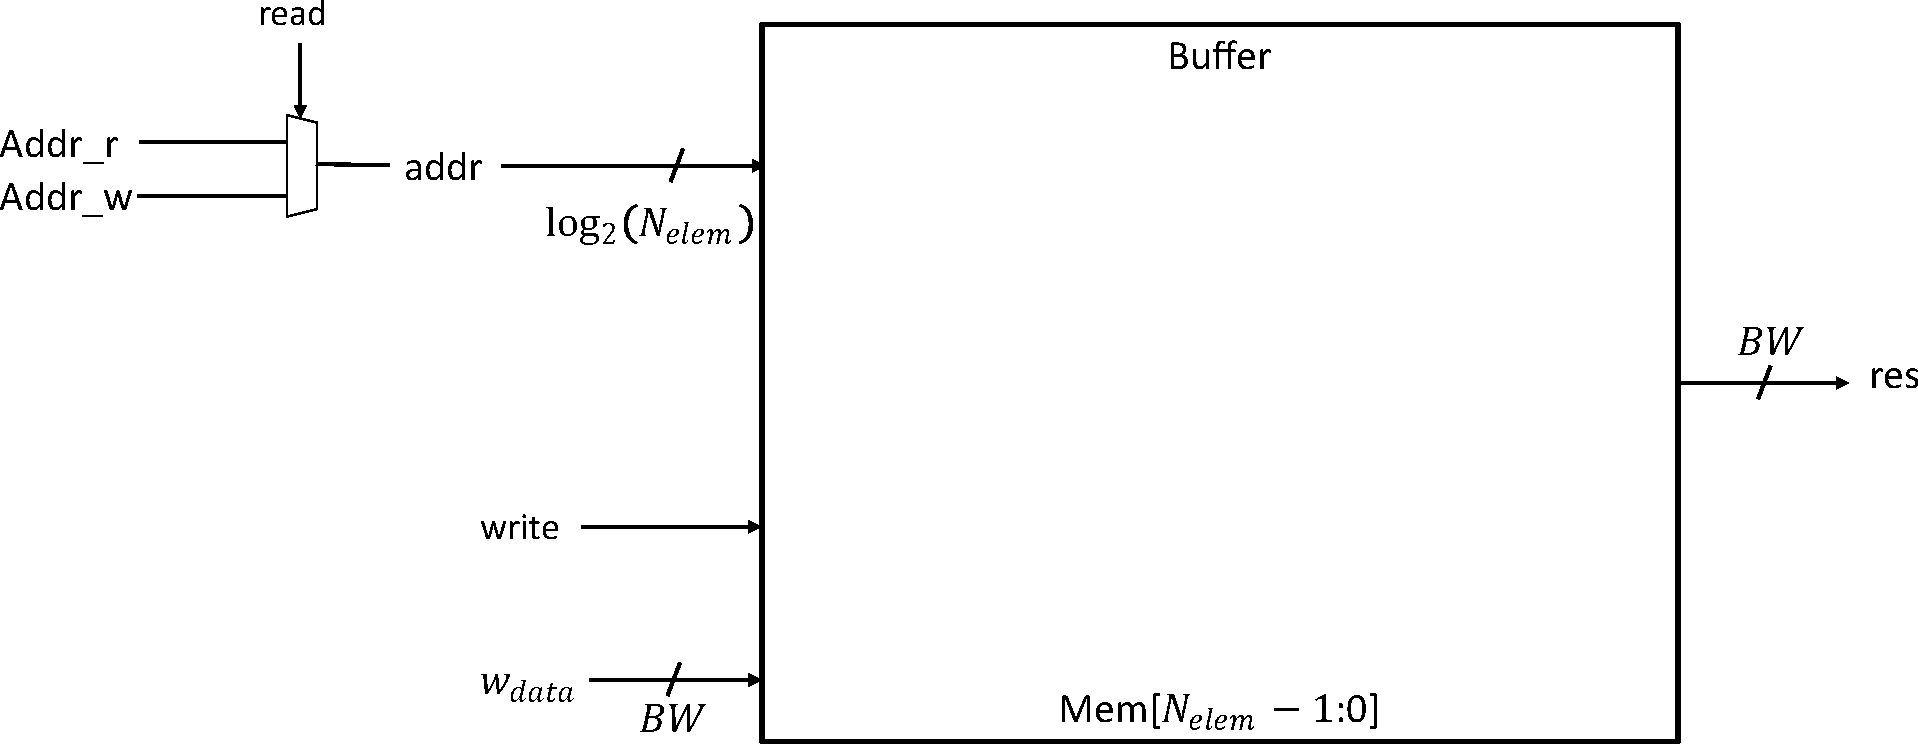
\includegraphics[width=\textwidth]{struct_ram.pdf}
    \caption{General architecture of a buffer component}
    \label{fig:struct_ram}
\end{figure}
%
The buffers compose the on-chip memory of the \acrshort{fpga}. As mentionned previously, the structure is composed of six buffers that share the same structure, as illustrated in Figure \ref{fig:struct_ram}. At each clock period, the output signal $res$ is equal to the value stored at address $addr$, or if the write signal $write$ is enabled, the value that is currently written. In the same way, if the write signal is set, the value in the buffer at address $addr$ is equal to the input data $w_{data}$. As multiple components may read or write a same buffer, a multiplexer is added to select from which address to read.

The value of $addr_r$ and $addr_w$ depend on the type of buffer. For \textbf{data buffer} the $addr_r$ is the \acrshort{pe} address of the corresponding buffer, and $addr_w$ is the \acrshort{dma} $ram_{addr}$ signals. For \textbf{result buffer}, $addr_w$ is the corresponding \acrshort{pe} output address and $addr_r$ can be either a \acrshort{pe} address requesting a result (\textbf{FMINT Buffer}) or the \acrshort{dma} $ram_{addr}$ signals to write final results to external memory ((\textbf{FMO Buffer}))

However, the differences between each buffer are the maximum number of elements that can be stored $N_{elem}$ and the bitwidth $BW$ of their data stored. We explore for each buffer these two parameters.
\begin{itemize}
    \item \textbf{FMI Buffer}: we have determined from the loops analysis that we buffer each input \acrshort{fm} fetching group. Since the number of input \acrshort{fm} channels vary accross the different layers of the network, we can determine $N_{elem}$ using Equation \eqref{eq:nelem-fmi}. The number of bits to store a pixel is equal to $BW_{pixel}$. We can therefore express $BW$ such as Equation \eqref{eq:bw-fmi}.
    \begin{equation}
        N_{elem-fmi} = \forall l \in layers: Max\left( N_{if}^l \times Min\left(T_{ix}, N_{ix}^l\right) \times Min\left(T_{iy}, N_{iy}^l\right) \right)
        \label{eq:nelem-fmi}
    \end{equation}
    \begin{equation}
        BW_{fmi} = BW_{pixel}
        \label{eq:bw-fmi}
    \end{equation}
    %
    \item \textbf{KEX Buffer}: this buffer stores the $N_{par}$ $1 \times 1$ kernels required to perform this convolution, which expands the number of input channels. Therefore, we can express $N_{elem}$ using Equation \eqref{eq:nelem_kex}, where $N_{gr-max} = \left\lceil \frac{1280}{Npar} \right\rceil$ is the maximum number of fetching group in the whole network. Since the weights are expressed in the proposed compressed format, we also have to store the weight position in the fetching group.
    As a result, $BW$ can be expressed using Equation \eqref{eq:bw-kex}, where $BW_{weight}$ is the number of bits to represent a weight and $log_2(N_{par})$ the number of bits to represent the position.
    \begin{equation}
        N_{elem-kex} = N_{par} \times N_{np} \times N_{gr-max}
        \label{eq:nelem_kex}
    \end{equation}
    \begin{equation}
        BW_{kex} = BW_{weight} + log_2(N_{par})
        \label{eq:bw-kex}
    \end{equation}
    %
    \item \textbf{FMINT Buffer}: since the \acrshort{dsc} needs $N_{par}$ intermediate \acrshort{fm} channels and the $1 \times 1$ convolution does not reduce the spatial dimension of the input \acrshort{fm}, we can express the $N_{elem}$ using Equation \eqref{eq:nelem_fmint}. The bitwidth of a pixel is the bitwidth used to represent a pixel, as in Equation \eqref{eq:bw-fmint}.
    \begin{equation}
        N_{elem-fmint} = N_{par} \times T_{iy} \times T_{ix}
        \label{eq:nelem_fmint}
    \end{equation}
    \begin{equation}
        BW_{fmi} = BW_{pixel}
        \label{eq:bw-fmint}
    \end{equation}
    %
    \item \textbf{KDW Buffer}: applying the same methodoly as \textbf{FMINT Buffer} and since the depthwise kernels are fully buffered, we can express the $N_{elem}$ using Equation \eqref{eq:nelem_kdw}. The bitwidth of a pixel is the bitwidth used to represent a weight, as in Equation \eqref{eq:bw-kdw}.
    \begin{equation}
        N_{elem-kdw} = N_{par} \times N_{ky} \times N_{kx}
        \label{eq:nelem_kdw}
    \end{equation}
    \begin{equation}
        BW_{kdw} = BW_{weight}
        \label{eq:bw-kdw}
    \end{equation}
    %
    \item \textbf{KPW Buffer}: for each time we perform a \acrshort{dsc}, we need to convolve in each pointwise the corresponding weight fetching group with $N_{np}$ pixels in the $N_{par}$ channels. The maximum number of elements in the buffer can be computed using Equation \eqref{eq:nelem_kpw}. As the pointwise convolution is a $1 \times 1$ convolution, the bitwidth associated to each pointwise kernel is the same as the \textbf{KPW Buffer}, and can be expressed using Equation \ref{eq:bw-kpw}
    \begin{equation}
        N_{elem-kpw} = N_{np} \times N_{of}
        \label{eq:nelem_kpw}
    \end{equation}
    \begin{equation}
        BW_{kpw} = BW_{weight} + log_2(N_{par})
        \label{eq:bw-kpw}
    \end{equation}
    %
    \item \textbf{FMO Buffer}: using the same methodoly as for determining $N_{elem}$ and $BW$ for the \textbf{FMI Buffer}, they are expressed using Equation \eqref{eq:nelem_fmo} and \eqref{eq:bw_fmo}
    \begin{equation}
        N_{elem-fmo} = \forall l \in layers: Max\left( N_{of}^l \times Min\left(T_{oy}, N_{oy}^l\right) \times Min\left(T_{ox}, N_{ox}^l\right) \right)
        \label{eq:nelem_fmo}
    \end{equation}
    \begin{equation}
        BW_{fmo} = BW_{pixel}
        \label{eq:bw_fmo}
    \end{equation}
\end{itemize}
